\documentclass{standalone}
\usepackage[dvipsnames]{xcolor}
\usepackage{tikz}
%\usepackage{pgfplots}
%\usepackage{pgfplotstable}
%\pgfplotsset{compat=1.5}
\usetikzlibrary{patterns}
\tikzstyle{v par}=              [dash pattern=on 10pt off 5pt,color=red!70,line width = 2pt]
\tikzstyle{z direction}=      [dash pattern=on 10pt off 5pt on 2pt off 5pt, color=Blue,line width = 2pt]

\begin{document}
{
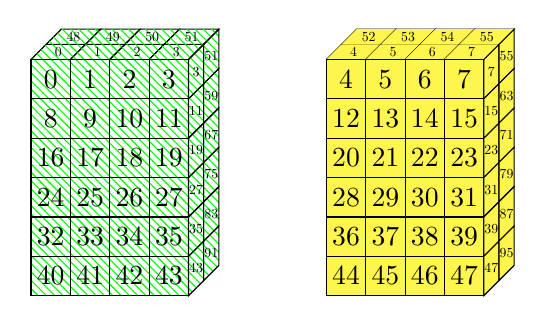
\begin{tikzpicture}
 \begin{scope}[scale=0.5]
 \def\nx{8}
\def\ny{2}
\def\nz{6}
 
 \pgfmathsetmacro\nxMax{\nx-1}
 \pgfmathsetmacro\nyMax{\ny-1}
 \pgfmathsetmacro\nzMax{\nz-1}
 
 \pgfmathsetmacro\nxSplit{int(\nx/2)}
 \pgfmathsetmacro\nySplit{int(\ny/2)}
 \pgfmathsetmacro\nzSplit{int(\nz/2)}
 
 \pgfmathsetmacro\nxSplitMax{\nxSplit-1}
 \pgfmathsetmacro\nySplitMax{\nySplit-1}
 \pgfmathsetmacro\nzSplitMax{\nzSplit-1}
 
 
 \foreach \x in {0,...,\nxSplitMax}
 {
  \pgfmathsetmacro\xVal{int(\x)}
  \foreach \z in {0,...,\nyMax}
  {
   \pgfmathsetmacro\yVal{int(\z)}
   \pgfmathsetmacro\zVal{0}
   \draw (\x,0,-\z) -- (\x,0,-\z-1) -- (\x+1,0,-\z-1) -- (\x+1,0,-\z);
   \fill[pattern=north west lines, pattern color=green] (\x,0,-\z) -- (\x,0,-\z-1) -- (\x+1,0,-\z-1) -- (\x+1,0,-\z);
   \pgfmathsetmacro\n{int(\xVal+\nx*\nz*\yVal+\nx*\zVal)}
   \node[scale=0.5] at (\x+0.5,0,-\z-0.5) {\n};
  }
  \foreach \y in {0,...,\nzMax}
  {
   \pgfmathsetmacro\zVal{int(\y)}
   \pgfmathsetmacro\yVal{0}
   \fill[pattern=north west lines, pattern color=green] (\x,-\y,0) rectangle (\x+1,-\y-1,0);
   \draw (\x,-\y,0) -- (\x,-\y-1,0) -- (\x+1,-\y-1,0) -- (\x+1,-\y,0) -- (\x,-\y,0);
   \pgfmathsetmacro\n{int(\xVal+\nx*\nz*\yVal+\nx*\zVal)}
   \node at (\x+0.5,-\y-0.5,0) {\n};
  }
 }
 
 \foreach \y in {0,...,\nzMax}
 {
  \pgfmathsetmacro\zVal{int(\y)}
  \pgfmathsetmacro\xVal{\nxSplitMax}
  \foreach \z in {0,...,\nyMax}
  {
   \pgfmathsetmacro\yVal{int(\z)}
   \fill[pattern=north west lines, pattern color=green] (\nxSplit,-\y,-\z) -- (\nxSplit,-\y,-\z-1) -- (\nxSplit,-\y-1,-\z-1) -- (\nxSplit,-\y-1,-\z) -- (\nxSplit,-\y,-\z);
   \draw (\nxSplit,-\y,-\z) -- (\nxSplit,-\y,-\z-1) -- (\nxSplit,-\y-1,-\z-1) -- (\nxSplit,-\y-1,-\z) -- (\nxSplit,-\y,-\z);
   \pgfmathsetmacro\n{int(\xVal+\nx*\nz*\yVal+\nx*\zVal)}
   \node[scale=0.5] at (\nxSplit,-\y-0.5,-\z-0.5) {\n};
  }
 }
  
  
  \begin{scope}[xshift=3.5cm]
    \foreach \x in {\nxSplit,...,\nxMax}
    {
      \pgfmathsetmacro\xVal{int(\x)}
      \foreach \z in {0,...,\nyMax}
      {
	\pgfmathsetmacro\yVal{int(\z)}
	\pgfmathsetmacro\zVal{0}
	\draw (\x,0,-\z) -- (\x,0,-\z-1) -- (\x+1,0,-\z-1) -- (\x+1,0,-\z);
	\fill[yellow!70] (\x,0,-\z) -- (\x,0,-\z-1) -- (\x+1,0,-\z-1) -- (\x+1,0,-\z);
	\pgfmathsetmacro\n{int(\xVal+\nx*\nz*\yVal+\nx*\zVal)}
	\node[scale=0.5] at (\x+0.5,0,-\z-0.5) {\n};
      }
      \foreach \y in {0,...,\nzMax}
      {
        \pgfmathsetmacro\zVal{int(\y)}
        \pgfmathsetmacro\yVal{0}
	\fill[yellow!70] (\x,-\y,0) rectangle (\x+1,-\y-1,0);
	\draw (\x,-\y,0) -- (\x,-\y-1,0) -- (\x+1,-\y-1,0) -- (\x+1,-\y,0) -- (\x,-\y,0);
	\pgfmathsetmacro\n{int(\xVal+\nx*\nz*\yVal+\nx*\zVal)}
	\node at (\x+0.5,-\y-0.5,0) {\n};
      }
    }
    
    \foreach \y in {0,...,\nzMax}
    {
      \pgfmathsetmacro\zVal{int(\y)}
      \pgfmathsetmacro\xVal{\nxMax}
      \foreach \z in {0,...,\nyMax}
      {
        \pgfmathsetmacro\yVal{int(\z)}
	\fill[yellow!70] (\nx,-\y,-\z) -- (\nx,-\y,-\z-1) -- (\nx,-\y-1,-\z-1) -- (\nx,-\y-1,-\z) -- (\nx,-\y,-\z);
	\draw (\nx,-\y,-\z) -- (\nx,-\y,-\z-1) -- (\nx,-\y-1,-\z-1) -- (\nx,-\y-1,-\z) -- (\nx,-\y,-\z);
	\pgfmathsetmacro\n{int(\xVal+\nx*\nz*\yVal+\nx*\zVal)}
	\node[scale=0.5] at (\nx,-\y-0.5,-\z-0.5) {\n};
      }
    }
    
  \end{scope}
 \end{scope}
\end{tikzpicture}
}
\end{document}
